\documentclass[11pt]{article}
\fontfamily{Times}

\usepackage[left=2cm,right=2cm,text={17cm, 24cm},top=2.cm]{geometry}
\usepackage[czech]{babel}
\usepackage[utf8x]{inputenc}
\usepackage{scrextend}
\usepackage{lipsum}
\usepackage{graphicx}
\usepackage{amsthm}
\usepackage{color}

%\usepackage{titlesec}
%\titlespacing\section{0pt}{12pt plus 4pt minus 2pt}{10pt plus 2pt minus 2pt}
%\titlespacing\subsection{20pt}{12pt plus 4pt minus 2pt}{10pt plus 2pt minus 2pt}
%\titlespacing\subsubsection{40pt}{12pt plus 4pt minus 2pt}{10pt plus 2pt minus 2pt}

\title{Počítačové komunikace a sítě\\[0.5 cm] Dokumentace k projektu 2}		
\author{Marek Kovalčík}								
\date{4. duben 2018}								

\makeatletter
\let\thetitle\@title
\let\theauthor\@author
\let\thedate\@date
\makeatother

\usepackage{tocloft}
\usepackage{changepage}


\renewcommand\cfttoctitlefont{\hfill\Large\bfseries}
\renewcommand\cftaftertoctitle{\hfill\mbox{}}


\setcounter{tocdepth}{2}

\begin{document}
	
	%%%%%%%%%%%%%%%%%%%%%%%%%%%%%%%%%%%%%%%%%%%%%%%%%%%%%%%%%%%%%%%%%%%%%
	
	\begin{titlepage}
		\centering
		\vspace*{0.5 cm}
		
\includegraphics[scale = 0.3]{img/logo.png}\\[2.0 cm]
		\textsc{\LARGE Vysoké učení technické v Brně}\\[0.3 cm]
		\textsc{\Large Fakulta informačních technologií}\\[2.0 cm]
		\rule{\linewidth}{0.2 mm} \\[2.0 cm]
		{ \huge \bfseries \thetitle}\\[2.0 cm]
		\LARGE{Varianta 1: Bandwidth Measurement}\\[0.5 cm]
		\rule{\linewidth}{0.2 mm} \\[2.0 cm]
		
		\begin{minipage}{0.4\textwidth}
			\begin{flushleft} \large
				\vspace{1 cm}
				Marek Kovalčík
			\end{flushleft}
		\end{minipage}
		\begin{minipage}{0.4\textwidth}
			\begin{flushright} \large
				%\emph{Login a ID:} 
				\vspace{1 cm}
				xkoval14, 196248 \hspace{1 cm}\\								
			\end{flushright}
		\end{minipage}\\[2 cm]
		
		{\large \thedate}\\[2 cm]
		
		\vfill
		
	\end{titlepage}
	%%%%%%%%%%%%%%%%%%%%%%%%%%%%%%%%%%%%%%%%%%%%%%%%%%%%%%%%%%%%%%
	\newpage
	\tableofcontents
	\clearpage
	
	
	%%%%%%%%%%%%%%%%%%%%%%%%%%%%%%%%%%%%%%%%%%%%%%%%%%%%%%%%%%%%%%
	
	\section{Zadání}
	\begin{flushleft}
		Cílem aplikace je pomocí vhodné komunikace změřit dostupnou přenosovou rychlost mezi dvěma stanicemi v Internetu. Pro měření se bude používat generovaná komunikace protokolu UDP. Tato aplikace se bude skládat ze dvou částí - Reflektoru a Měřáku. Měření bude probíha pomocí zasílání UDP paketů tkz. sond z měřáku na reflektor. Reflektor pouze odpovídá na příchozí sondy. Měřák musí implementovat vhodný algoritmus pro zjištění maximální přenosové rychlosti - tedy zjistit jak rychle je možné sondy posílat aniž by docházelo ke ztrátě paketů. Návrh tohoto algoritmu je hlavním výstupem teoretické části projektu.\par		
		
		\begin{center}
			Spuštění reflektoru (server): ./ipk-mtrip reflect -p port\\[0.5 cm]
			\begin{itemize}
				\item argument 'reflect' označuje, že aplikace bude spštěna jako reflektor
				\item -p PORT: určuje číslo portu, na němž reflektor poběží
			\end{itemize}
		\end{center}
		\begin{center}
			Spuštění meřáku (klient): ./ipk-mtrip meter -h HOST -p PORT -s SONDA -t TIME  \\[0.5 cm]
			\begin{itemize}
				\item argument 'meter' označuje, že aplikace bude spuštěna jako meřák
				\item -h HOST: IP adresa nebo doménové jméno vzdáleného počítače, na němž běží ipk-mtrip spuštěn jako reflektor
				\item -p PORT: číslo portu, na kterém reflektor naslouchá
				\item -s SONDA: určuje velikost zprávy k měření
				\item -t TIME: určuje čas v sekundách, po který se bude měřit
			\end{itemize}
		\end{center}
		
		Výsledkem měření je výpis informací o měření na standardní výstup. Součástí výstupních informací je průměrná naměřená přenosová rychlost, maximální naměřená přenosová rychlost, minimální naměřená přenosová rychlost, standardní odchylka naměřených rychlostí a průměrný RTT paketů komunikace.
			
	\end{flushleft}
	
	\section{Trocha teorie}
	\begin{flushleft}
		Šířka pásma (bandwith) je frekvenční interval rozsahu přenášeného elektromagnetického signálu v rádiových technologií. V IT světě zase udává objem datových bloků, které dané zařízení dokáže za jistý čas přenést dále.[1]\\[0.5 cm] 	
		Obousměrné zpoždění (Round-tip-time, RTT) označuje čas kdy paket je odeslán na specifický cíl a navrácen zpět. V tomto projektu a mnohých dalších zdrojích je RTT uváděno v milisekundách.[2]	
	\end{flushleft}
	
	\newpage
	\section{Popis implementace}
		\begin{flushleft}
			Na začátku programu jsou zkontrolovány vstupní parametry a pokud neodpovídají očekávaným parametrům včetně validních hodnot, program je ukončen. V opačném případě se provede spuštění reflektoru či metru. Jsou-li argumenty zadány špatně, vypíše se nápověda k programu.
		\end{flushleft}
		\subsection{Implemetace reflektoru}
			\begin{flushleft}
				Je-li aplikace spuštěna jako server, vytvoří se socket a reflektor přejde do stavu "čekání". Spustí se nekonečná smyčka, ve které server čeká na příchozí pakety od klienta. Jakmile ho obdrží, zase mu jej pošle zpátky a mezitím si počítá kolik, paketů mu již došlo. Jakmile reflektoru dojde paket s obsahem "$konec\_spojeni$", odešle zpět klientovi informaci o počtu úspěšně přijatých paketů a své interní počítadlo vynuluje.\\[0.5 cm]	
				Činnost reflektoru běží v nekonečné smyčce a pro ukončení programu se využívá signál SIGKILL (CTRL+C)\par	
			\end{flushleft}
			
		\subsection{Implementace měřáku}
			\begin{flushleft}
				Měření je implementováno tak, že meter ve smyčce odesílá pakety na reflektor tak rychle, jak mu to operační systém dovolí a počítá si kolik jich již odeslal.\\[0.5 cm]
				Je-li zadaný čas 1 vteřina, provádí se jeden cyklus po dobu jedné vteřiny. Hlídání času je zajištěno pomocí alarmů. Je-li zadaný čas 2,3 nebo 4 vteřiny, provádí se 2,3 nebo 4 cykly s odesíláním paketů na reflektor, každý po dobu jedné vteřiny. Je-li zadaný čas větší než 4 vteřiny, provádí se 5 cyklů. První čtyři po dobu jedné vteřiny a pátý cyklus po dobu t-4 vteřin.\\[0.5 cm]
				V každém cyklu je do pole přijatých zpráv přidán záznam o počtu úspěšně přijatých zpráv reflektorem získaný odesláním $konec\_spojeni$. Jelikož, meter ví, jak dlouho každý cyklus probíhal, dokáže vypočítat z těchto dat jednotlivé rychlosti, které se uloží do pole naměřených rychlostí.\\[0.5 cm]
				Z pole naměřených rychlostí se pak pomocí jednoduchých pomocných funkcí získá průměrná, maximální, minimální naměřená rychlost a standardní odchylka.\\[0.5 cm]
				Měření obousměrného zpoždění probíhá v prvním cyklu měření a je implementováno tak, že funkce sendto() a recv() se zabalí mezi začátek gettimeofday() a konec gettimeofday(). Tato funkce do svých parametrů uloží údaje o čase potřebném pro vykonání jednoho sendto() a recv(). Z těchto údajů se potom vypočítá potřebný čas v milisekundách a opět uloží do pole naměřených časů, ze kterého se na konec udělá průměr pro výpis informace na standardní výstup.
							
			\end{flushleft}	

	
	%%%%%%%%%%%%%%%%%%%%%%%%%%%%%%%%%%%%%%%%%%%%%%%%%%%%%%%%%%%%%%
	\newpage		
	\section{Přílohy}
			Reflektor i meter jsem testoval v mnoha varintách. Spuštění serverové i klientské aplikace na domácím počítači, spuštění serveru na vzdáleném serveru a klienta na domácím počítači nebo spuštění obou aplikací na vzdáleném serveru. Výstupy fungovaly tak jak měly, avšak pro přehlednost a stručnost dokumentace zde uvádím jen pár demonstračních příkladů.
		\subsection{Make na serveru merlin.fit.vubr.cz}
	\begin{center}
		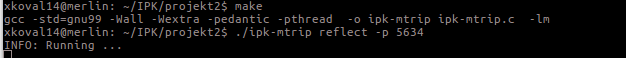
\includegraphics[scale = 0.8]{img/makeMerlin.png}\\
	\end{center}

	\subsection{Měření z localhostu reflektováno serverem merlin.fit.vutbr.cz}
	\begin{center}
		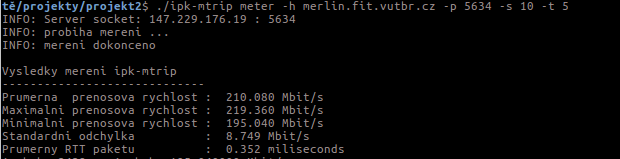
\includegraphics[scale = 0.83]{img/mereniMerlin.png}\\
	\end{center}
	
	\subsection{Měření z localhostu reflektováno serverem eva.fit.vutbr.cz}
	\begin{center}
		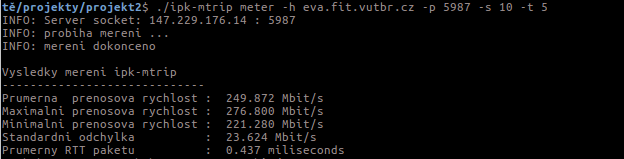
\includegraphics[scale = 0.83]{img/mereniEva.png}\\
	\end{center}
	\newpage
	\subsection{Měření z merlin.fit.vutbr.cz reflektováno serverem eva.fit.vutbr.cz}
	\begin{center}
		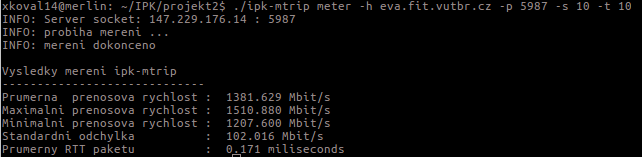
\includegraphics[scale = 0.76]{img/mereniMerlinEva.png}\\
	\end{center}
	\subsection{Měření z eva.fit.vutbr.cz reflektováno serverem merlin.fit.vutbr.cz}
	\begin{center}
		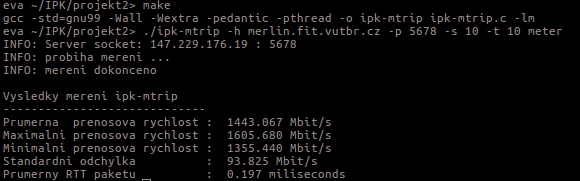
\includegraphics[scale = 0.83]{img/mereniEvaMerlin.png}\\
	\end{center}
	

	
	\vfill
	%%%%%%%%%%%%%%%%%%%%%%%%%%%%%%%%%%%%%%%%%%%%%%%%%%%%%%%%%%%%%%
	
	\section{Použité zdroje}
	\begin{flushleft}
		[1] Co je šířka pásma, SPRÁVA SÍTĚ [online]. upraveno 2016, [cit. 2018.04.04] Dostupné z: https://www.sprava-site.eu/sirka-pasma/\par
		
		[2] Round-trip-time, Network management and monitoring. The evolution of network control [online], upraveno. neuvedeno, [cit. 2018-04-04], Dostupné z: https://searchnetworking.techtarget.com/definition/round-trip-time
		
		[3] Demonstrační soubory, Demo\_C.zip [online]. upraveno: 2018-02-22 [cit. 2018-04-04]. Dostupné z: https://wis.fit.vutbr.cz/FIT/st/course-files-st.php?file=\%2Fcourse\%2FIPK-IT\%2Fother\&cid=11963\par	
	\end{flushleft}	

\end{document}